% !TeX spellcheck = de_DE
\documentclass[a4paper,12pt]{report}
% es wurde leqno entfernt, da damit die Nummern von Gleichungen links standen
\usepackage{inputenc,fontenc}
\usepackage[a4paper,margin=3cm]{geometry}
\usepackage[english, german]{babel}
\usepackage[ngerman=ngerman]{hyphsubst}
% \usepackage{isodate}
\usepackage[hidelinks]{hyperref}
\usepackage{amsmath, amsfonts, amssymb, amsthm} %% mathematics tools
\usepackage{csquotes}
\usepackage[draft]{listofsymbols}
\usepackage[backend=biber, urldateusetime=true, sorting=none]{biblatex} %% Literature citing engine
\usepackage{subcaption}
\usepackage{graphicx}
\usepackage{dsfont} % für charakteristische 1

%%
%% Pflichtangaben -bitte hier einsetzen %%%%%%%%%%%%%%%%%%%%%%%%%%%%%%%%%%%%%%%%%%%%%%
%%
\newcommand{\name}{Göpel}
\newcommand{\vorname}{Noah}
\newcommand{\gebdatum}{01.02.2003}
\newcommand{\ort}{Riesa}
\newcommand{\betreuer}{Prof. Dr. Oliver Sander}
\newcommand{\institut}{Institut für Numerische Mathematik}
\newcommand{\thema}{Gewichtete Eigenwert-Zählung auf einem Intervall}
\newcommand{\datum}{tt.\ mm.\ jjjj} %Format tt.\ mm.\ jjjj

%%%%%%%%%%%%%%%%%%%%%%%%%%%%%%%%%%%%%%%%%%%%%%%%%%%%%%%%%%%%%%%%%%%%%%%%%%%%%%%%%%%%%%


%__________Definitions_____________________________

% Literaturverzeichnis
\addbibresource{Literatur.bib}
\graphicspath{{src/}}

% \newcommand{\bild}[2]{\includegraphics[width=#2\textwidth,height=#2\textheight,keepaspectratio]{#1}}
\newcommand{\bild}[4]{
      \begin{figure}[!htp]
            \centering
            \includegraphics[width=#2\textwidth,height=#2\textheight,keepaspectratio]{#1}
            \caption{#3}
            #4
      \end{figure}
}
\newcommand{\R}{\mathbb R}
\newcommand{\C}{\mathbb C}
\newcommand{\zitat}[1]{\glqq #1 \grqq}
\newcommand{\klammer}[1]{\left(#1\right)}
\newcommand{\diag}{\text{diag}}
\newcommand{\rang}{\text{rang}}
\newcommand{\tr}{\text{tr}}
\newcommand{\AlamB}{A-\lambda\,B}
\newcommand{\Cnn}{\C^{n\times n}}
\newcommand{\inv}{^{-1}}
\newcommand{\1}{\mathds{1}}

% wird für Symbolverzeichnis benutzt, sonst gibt es Fehler
\DeclareOldFontCommand{\bf}{\normalfont\bfseries}{\mathbf}

% Math
\theoremstyle{plain} % text is cursive
\newtheorem{theorem}{Theorem}
\newtheorem{lemma}[theorem]{Lemma}  %% [theorem] means same numbering for theorem and lemma
\newtheorem{proposition}[theorem]{Proposition}
\newtheorem{corollary}[theorem]{Korollar}

\theoremstyle{definition} % text is "upright"
\newtheorem{definition}[theorem]{Definition}
\newtheorem{example}[theorem]{Beispiel}

\theoremstyle{remark}
\newtheorem{remark}[theorem]{Bermerkung}

% Symbolverzeichnis
\renewcommand{\symheadingname}{Symbolverzeichnis}
\opensymdef
      % \newsym[]{}{}
      \newsym[Einheitsmatrix]{In}{I_n}
      \newsym[Massenmatrix]{M}{M}
      \newsym[Steifigkeitsmatrix]{K}{K}
      \newsym[Federkraft]{FL}{\overrightarrow{F_L}}
      \newsym[Trägheitskraft]{FT}{\overrightarrow{F_T}}
      \newsym[Verschiebung des k-ten Massepunktes aus der Ruhelage]{xk}{x_k}
      \newsym[Eigenkreisfrequenz]{w}{\omega}
\closesymdef


\begin{document}
\selectlanguage{german}

%% Titelseite
\thispagestyle{empty}

\begin{center}
{\Large Technische Universit\"{a}t Dresden\  \ \textbullet\ \ Fakult\"{a}t Mathematik}

\vfil

{\bfseries\Huge\thema}

\vfil
{\LARGE
Bachelorarbeit \\[\bigskipamount]
zur Erlangung des ersten Hochschulgrades\\[\bigskipamount]
\bfseries{\itshape Bachelor of Science  \textup{(}B.Sc.\textup{)}}\\[\bigskipamount]
}

\vfil\vfil

\vfil

vorgelegt von
\\[\bigskipamount]
\textsc{\vorname\ } \MakeUppercase{\name}
\\[\bigskipamount]
(geboren am \gebdatum\ in \textsc{\ort})
\\[\bigskipamount]
Tag der Einreichung: \datum
\\[\bigskipamount]
\betreuer\ (\institut)
\end{center}

\cleardoublepage
%%%%%%%%%%%%%%%%%%%%%%Beginn Ausarbeitung%%%%%%%%%%%%%%%%%%%%%%%%%%%%%%%%
\tableofcontents
\clearpage
\listofsymbols
\clearpage

\chapter{Einleitung}
\label{sec: Einleitung}
      
      Diese Ausarbeitung beschäftigt sich mit numerischen Verfahren, um sicherzustellen, dass für ein gegebenes mechanisches System keine Eigenwerte in einem vorgegebenem festen Intervall liegen.
% hier muss noch einiges getan werden
      Damit kann sichergestellt werden, dass die Eigenfrequenzen des Systems nicht so liegen, dass es zu einer Selbsterregung kommt.

      % Um diese Anforderung zu erfüllen, werden die Eigenwerte des Matrix Pencils auf diesem Intervall gewichtet gezählt. Man erhält ein Minimierungsproblem,
      % in welchem es gilt, einen Design-Paramerter so anzupassen, dass auf dem Intervall kein Eigenwert des entsprechenden Systems mehr vorhanden ist.
      % Dazu werden in den Kapiteln \ref{sec: MS Matrizen} und \ref{sec: EW Problem} die theoretischen Grundlagen gelegt.
      % Anschließend werden in Kapitel \ref{sec: Quellen} die entscheidende Identität von Futamura und wichtige Überlegungen ausgeführt.

      % Daraufhin werden diese Überlegungen in Kapitel \ref{sec: Programmieren} anhand verschiedener Beispiele implementiert und getestet.

      Die Auswertung und Verbesserung der Implementation folgt in Kapitel \ref{sec: Verbesserungen}.

      % In dieser Ausarbeitung werden die gewichtete Zählung von Eigenwerten auf einem Intervall behandelt, um sicherzustellen,
      % dass bei einem vorgegebenem mechanischem System keine Eigenwerte in einem bestimmten festen Intervall liegen.
      % Dazu wird in den ersten Kapiteln die nötige Theorie anhand der Quellen \cite{grundlageFutamura} und \cite{hauptteilTkachuk} beschrieben.
      % Hier werden Matrix Pencil und das verallgemeinerte Eigenwertproblem verwendet, um 
      % Hierzu nutzt man die Identität von Futamura, um die Zählung der Eigenwerte auf die zugrundeliegenden Matrizen zurückzuführen.


      % und anschließend in Kapitel \ref{sec: Programmieren} in Python angewendet.
      % Daraufhin werden in Kapitel \ref{sec: Verbesserungen} die Ergebnisse kritisch betrachtet und weitere Algorithmen eingeführt, um die Berechnungen zu beschleunigen.
      Zum Schluss werden in Kapitel \ref{sec: Auswertung} die Ergebnisse wiederholt und ein Ausblick in weiterführende Themen gegeben.

      Ferner werden in Kapitel \ref{sec: Verbesserungen} eine Approximation der Matrix-Spur vorgestellt und ebenfalls implementiert.

\chapter{Das verallgemeinerte Eigenwert-Problem und die Identität von Futamura}
\label{sec: EW Problem_Futamura}

      Zu Beginn der Ausarbeitung werden einige Resultate über Matrizen und lineare Algebra behandelt.
      Diese werden in Kapitel \ref{sec: EW Zählung} verwendet, um die Zählung der Eigenwerte zu einer differenzierbaren Funktion umzustellen.
      
      \section{Der Matrix Pencil}
            Betrachte zunächst das Konzept des Matrix Pencil, welches in dieser Ausarbeitung eine entscheidende Rolle spielt.
            \begin{definition}(pencil, \cite[S. 375]{matrixGolub})
                  \label{def: pencil}
                  Seien $A$ und $B$ Matrizen in $\C^{n\times n}$, dann wird die Menge aller Matrizen der Form
                  $\AlamB, \lambda \in \C$ pencil genannt.
            \end{definition}

            Laut \cite[S. 375]{matrixGolub} seien die Eigenwerte von $\AlamB$ diejenigen $\lambda \in\C$, für die gelte:
            \begin{equation}
                  \label{eqn: verallg EW Problem}
                  (\AlamB)x=0,\quad x\ne 0
            \end{equation}
            
            Hier wird $x\in\C^n$ Eigenvektor genannt.
            Man beachte, dass für $B=\In$ Gleichung (\ref{eqn: verallg EW Problem}) die folgende Form annimmt:
            $$(A-\lambda\In)x=0 \Leftrightarrow Ax = \lambda x,$$
            also genau die Definition des Eigenwert-Problems.
% gibt es ein Eigenwert-Problem und wenn ja, gibt es eine Definition? oder ist es einfach eine Gleichung?
            Daher wird die Suche nach den $\lambda\in\C$, die (\ref{eqn: verallg EW Problem}) erfüllen auch verallgemeinertes Eigenwert-Problem genannt, da sie eine allgemeine Form des speziellen Eigenwertproblems darstellen.

            Falls man $\AlamB$ durch die Matrix $C$ ersetzt, so entsteht aus (\ref{eqn: verallg EW Problem}) das lineare homogene Gleichungssystem
            $$Cx=0,\quad x\ne 0$$

            Nach einem Resultat aus der linearen Algebra gilt:
% welches Resultat?, ich habe es bis jetzt nur in Skript LA20 gefunden
            $$\det(C)\ne 0 \Leftrightarrow Cx=0 \text{ hat als einzige Lösung }x=0$$
            Durch Negation folgt:
            $$\det(C)=0 \Leftrightarrow \exists x\ne 0: Cx=0$$

            Somit sucht man die Eigenwerte des Pencils, in dem man die Nullstellen des Polynoms $\det(\AlamB)$ berechnet\footnote{Man könnte das Polynom $\det(\AlamB)$ als eine Art charakteristisches Polynom des Pencils $\AlamB$ betrachten, ähnlich dem charakteristischen Polynom $f(A)$ einer Matrix $A$}.
            
            Daher wird in \cite[S. 375]{matrixGolub} die Menge der Eigenwerte des Pencils $\AlamB$ wie folgt definiert:
            \begin{equation}
                  \label{def: EW Pencil}
                  \lambda(A,B):=\{z\in\C:\ \det(A - zB) = 0\}
            \end{equation}

%%%%%%%%%%%%%%%%%%%%%%%%%%%%%%%% Def regulärer pencil mit Quelle fehlt %%%%%%%%%%%%%%%%%%%%%%%%%%%%%%%%

%             Zum Schluss folgt noch eine Definition, welche in Kapitel \ref{sec: Futamura} benötigt wird:
%             \begin{definition}
%                   Ein Pencil heißt regulär, falls $B$ invertierbar ist.
%             \end{definition}
% % Quelle einfügen

%             Man beachte, dass für einen regulären Pencil gilt:
%             $$(\AlamB)x = 0 \Leftrightarrow (B^{-1}A - \lambda \In)x = 0$$
%             Weshalb $$\lambda(A,B) = \lambda(B^{-1}A,\In) = \lambda(B^{-1}A),$$
%             also kann man die Eigenwerte des regulären Pencils auf ein spezielles Eigenwertproblem zurückführen und die normalen Eigenwerte von $B^{-1}A$ sind genau die Eigenwerte des Pencils $\AlamB$.
      \section{Die Schur-Zerlegung}
            In diesem Kapitel werden weitere wichtige Konzepte vorgestellt, die für Kapitel \ref{sec: Futamura} benötigt werden.

            \begin{definition}(\cite[S. 73]{matrixGolub})
                  Sei $Q \in\C^{n\times n}$, dann wird $Q$ unitär genannt, wenn
                  $$Q^HQ = QQ^H=\In$$
            \end{definition}

            Hier ist $Q^H := \Bar{Q^T}$ die Adjungierte von $Q$, also die skalar komplex konjugierte Transponierte von $Q$.
% hier gibt es noch Verbesserungsmöglichkeiten

            Mithilfe dieser Definition können nun folgende Resultate behandelt werden:
            \begin{theorem}(Theorem 7.1.3 (Schur Decomposition)\cite[S. 313]{matrixGolub})
                  \label{thrm: Schur Zerlegung}
                  Wenn $A \in \C^{n\times n}$, dann existiert eine unitäre Matrix $Q\in\C^{n\times n}$, sodass
                  \begin{equation}
                        \label{eqn: Schur_Resultat}
                        Q^H\,AQ = T = D+N
                  \end{equation}
                  mit $D=\diag(\lambda_1,\dots,\lambda_n)$ und $N\in\C^{n\times n}$ strikter oberer Dreiecksmatrix.
                  Ferner kann $Q$ so gewählt werden, dass die Eigenwerte $\lambda_i$ in beliebiger Reihenfolge auf der Diagonalen auftauchen.
            \end{theorem}

% bessere Erlärung, warum spezielleres Lemma
            Um dieses Theorem zu beweisen, benötigt man ein Hilfslemma aus \cite[S.312]{matrixGolub}.
            Das Resultat wird hier in dem speziellen Fall vorgestellt, wie er für den Beweis von Theorem \ref{thrm: Schur Zerlegung} benötigt wird.

            \begin{lemma}(vgl. Lemma 7.1.2\cite[S. 312]{matrixGolub})
                  \label{lemma: Hilfe Schur}
                  Falls für $A\in\C^{n\times n}, \lambda\in \C \text{ Eigenwert von }A\text{ und }X\in \C^{n}$
                  \begin{equation}
                        \label{eqn: Hilfslemma Schur_Bed}
                        AX = X\lambda,\qquad \rang(X)=1
                  \end{equation}
                  
                  gilt, dann existiert ein $Q\in \C^{n\times n}$ unitär, sodass
                  $$Q^H\,AQ = T =  \begin{bmatrix}
                        \lambda & T_{12} \\
                        0 & T_{22} \\
                        \end{bmatrix}$$
                  mit $T_{22}\in \C^{(n-1)\times(n-1)}$
            \end{lemma}

            Beweis:
            Erhalte mit \cite[S. 233]{matrixGolub} eine komplexe QR-Zerlegung für $X$. Es gilt dann
            $$X = Q\ \begin{bmatrix}
                  r\\
                  0\\
                  \vdots\\
                  0
            \end{bmatrix}$$
            mit $Q\in \C^{n \times n}$ unitär und $r\in \C$.
            Durch Einsetzen in (\ref{eqn: Hilfslemma Schur_Bed}) und Multiplikation mit $Q^H$ folgt
            \begin{equation}
                  \label{eqn: Hilfslemma_Schur_Gl}
                  \underbrace{Q^H\,AQ}_{=:T}\ \begin{bmatrix}
                        r\\
                        0\\
                        \vdots\\
                        0
                  \end{bmatrix} = Q^H\,Q\ \begin{bmatrix}
                        r\\
                        0\\
                        \vdots\\
                        0
                  \end{bmatrix}\ \lambda
            \end{equation}
% man könnte hier R statt dem Vektor nutzen, dann wäre es kompakter
            mit $T:=\begin{matrix}
                  \begin{bmatrix}
                        T_{11} & T_{12}\\
                        T_{21} & T_{22}\\
                  \end{bmatrix} & \begin{matrix}
                  \text{\small 1} \\\text{\small{n-1}}
                  \end{matrix} \\
                  \begin{matrix}
                  \text{\small 1} &  \text{  \small{n-1}}\\
                  \end{matrix} &  \\
                  \end{matrix}$\\

                  
            Durch Ausmultiplizieren von (\ref{eqn: Hilfslemma_Schur_Gl}) folgen die Gleichungen\\

            $$\begin{aligned}
                  T_{11}\,r =& r\,\lambda\\
                  T_{21}\,r =& 0
            \end{aligned}$$

            mit $\rang(X)=1 \Rightarrow X\ne 0 \Rightarrow r\ne 0$ folgt $T_{11} = \lambda,\ T_{21} = 0$.\qed
% irgendwo muss erklärt werden, dass lam(A) = lam vereinigt lam(T_22)
            

            Nun können wir Theorem \ref{thrm: Schur Zerlegung} beweisen.


            Beweis Theorem \ref{thrm: Schur Zerlegung}(vgl. \cite[S. 313]{matrixGolub}):

            Offenbar gilt für $n=1$: $A$ ist ein Skalar, wodurch (\ref{eqn: Schur_Resultat}) für alle $Q$ unitär erfüllt ist.
            Sei nun $n>1$ und (\ref{eqn: Schur_Resultat}) gelte für alle $k<n$, dann gilt für einen beliebigen Eigenwert $\lambda$ von $A$:
            $$AX = \lambda X = X \lambda,\quad X\in \C^n, X\ne 0$$
            Nach Lemma \ref{lemma: Hilfe Schur} existiert $U\in \C^{n\times n}$, sodass
            $$U^H\, AU = \begin{bmatrix}
                  \lambda & T_{12} \\
                  0 & T_{22} \\
                  \end{bmatrix}$$
            Da aber $T_{22}\in\C^{(n-1)\times(n-1)}$, so gilt nach der Induktionsvoraussetzung:
            $$\widetilde U^H\,T_{22}\widetilde U = R,$$
            wobei $R\in\C^{(n-1)\times(n-1)}$  rechte obere Dreiecksmatrix, $\widetilde U \in\C^{(n-1)\times(n-1)}$ unitär.

            Sei nun $Q:=U\cdot\begin{bmatrix}
                  1&0\\
                  0&\widetilde U
            \end{bmatrix}$

            dann gilt mit\footnote{die folgende Gleichung stammt aus \cite{conjugateTranspose}, Beweis ebenfalls dort zu finden}
% Fussnote vielleicht scheisse platziert
            \begin{equation}
                  \label{eqn: Produkt Adjungierter}
                  \klammer{AB}^H = B^HA^H,\quad A,B\in \C^{n\times n}
            \end{equation}
            für (\ref{eqn: Schur_Resultat}):
            $$\begin{aligned}
                  Q^H\,AQ =& \begin{bmatrix}
                        1&0\\
                        0&\widetilde U
                  \end{bmatrix}^H\,U^H\,AU \begin{bmatrix}
                        1&0\\
                        0&\widetilde U
                  \end{bmatrix} = \begin{bmatrix}
                        1&0\\
                        0&\widetilde U^H
                  \end{bmatrix}
                  \begin{bmatrix}
                        \lambda & T_{12} \\
                        0 & T_{22} \\
                  \end{bmatrix}
                  \begin{bmatrix}
                        1&0\\
                        0&\widetilde U
                  \end{bmatrix}\\
                  =& \begin{bmatrix}
                        \lambda&T_{12}\\
                        0&\widetilde U^H\, T_{22}
                  \end{bmatrix}
                  \begin{bmatrix}
                        1&0\\
                        0&\widetilde U
                  \end{bmatrix}
                  = \begin{bmatrix}
                        \lambda&T_{12}\,\widetilde U\\
                        0&\widetilde U^H\, T_{22}\, \widetilde U
                  \end{bmatrix}\\
                  =& \begin{bmatrix}
                        \lambda&T_{12}\,\widetilde U\\
                        0&R
                  \end{bmatrix}
            \end{aligned}$$
            Wobei verwendet wurde, dass die komplex konjugierte skalar wirkt, also es gilt:
% vllt. Bullshit, am besten Beweis/Quelle finden
           
           \begin{equation}
            \label{eqn: Adjungierte reinziehen}
                  \begin{bmatrix}
                        1&0\\
                        0&\widetilde U
                  \end{bmatrix}^H = \overline{\begin{bmatrix}
                        1&0\\
                        0&\widetilde U^T
                  \end{bmatrix}} = \begin{bmatrix}
                        \overline{1}&0\\
                        0&\overline{\widetilde U^T}
                  \end{bmatrix} = \begin{bmatrix}
                        1&0\\
                        0&\widetilde U^H
                  \end{bmatrix}
           \end{equation}

            Damit ist gezeigt, dass $Q^H\,AQ$ eine rechte obere Dreiecksmatrix ist.
            Es fehlt noch zu zeigen, dass $Q$ unitär ist, dass kann aber mit (\ref{eqn: Produkt Adjungierter}) und (\ref{eqn: Adjungierte reinziehen}) einfach gezeigt werden.
            Die Beliebigkeit der Anordnung der Eigenwerte auf der Diagonalen folgt durch rekursives Anwenden von Theorem \ref{thrm: Schur Zerlegung} auf die Matrix $T_{22}$. \qed

            % Durch Lemma 7.1.1 aus \cite[S. 311]{matrixGolub} kann ferner gefolgert werden, dass die Diagonaleinträge genau die Eigenwerte sind.

            Nun wird eine weitere Schur-Zerlegung vorgestellt. Diese wird für den Beweis der Identität von Futamura in Kapitel \ref{sec: Futamura} benötigt.
%hier kann noch viel mehr erzählt werden: die Eigenschaft der Eigenwerte ist von entscheidender Relevanz
            \begin{theorem}(Generalized Schur Decompositon, \cite[S. 377]{matrixGolub})
                  \label{thrm: allg Schur Zerlegung}
                  Seien $A, B \in \C^{n\times n}$, dann existieren $Q$ und $Z$ unitär, sodass
                  \begin{equation}
                        \label{eqn: allg Schur_Resultat}
                        Q^H\,AZ = T,\quad Q^H\, BZ = S
                  \end{equation}
                  mit $T$ und $S$ obere Dreiecksmatrizen.
                  Falls für ein $k\in \{1,..., n\}\ t_{kk}=s_{kk}=0$, dann gilt $\lambda(A, B) = \C$, sonst
                  \begin{equation}
                        \label{eqn: EW Pencil nach Schur}
                        \lambda(A, B) = \{t_{ii}/s_{ii}:\, s_{ii}\ne 0\}
                  \end{equation}
            \end{theorem}
            Beweis: siehe \cite[S. 377]{matrixGolub}\qed

            

% k.A. ob das so stimmt
      
      \section{Die Identität von Futamura}
      \label{sec: Futamura}

            Nach den Vorbereitungen, die in diesem Kapitel gemacht wurden, kann nun die Identität von Futamura beschrieben und gezeigt werden.

            Das folgende Theorem wird für das Finden einer Zielfunktion von entscheidender Relevanz,
            da durch diese Aussage in Kapitel \ref{sec: EW Zählung} ein Zusammenhang zwischen der Anzahl der Eigenwerte und einem Integral über Matrizen gezeigt werden kann.

            \begin{theorem}
                  \label{thrm: IdentitätFutamura}(vgl. \cite[S. 127]{grundlageFutamura})
                  Seien $A, B\in\Cnn, z\in \C$, sodass $(zB-A)$ ein regulärer Matrix pencil ist, dann gilt:
                  \begin{equation}
                        \label{eqn: Resultat_Futamura}
                        \tr((zB-A)\inv B) = \sum_{j=1}^{n'} \frac{1}{z-\lambda_j},
                  \end{equation}
                  wobei $n'$ die Anzahl an von Null verschiedener Eigenwerte des pencils $(zB-A)$ und $\lambda_j$ die Eigenwerte des pencils sind.
%ist es die Anzahl von Null verschiedener Eigenwerte?
            \end{theorem}
% warum zB-A? für Eigenwerte macht es keinen Unterschied
            Beweis:
            Nach Theorem \ref{thrm: allg Schur Zerlegung} gibt es unitäre Matrizen $Q$ und $U\in\Cnn$, sodass nach entsprechender Multiplikation gilt:
            $$A=QTU^H,\quad B=QSU^H$$
            mit $T,S\in\Cnn$ obere Dreiecksmatrizen.
            
            Man kann folgern:
            \begin{align*}
                  (zB-A)\inv B =& (z\,QSU^H-QTU^H)\inv QSU^H = (Q(zS-T)U^H)\inv QSU^H \\
                  =& U(zS-T)\inv Q^H\,QSU^H = U(zS-T)\inv S\,U\inv
            \end{align*}
            wobei die Regel für Inverse von Matrixprodukten und die Definition von unitären Matrizen verwendet wurde.

            Man sieht, dass $(zB-A)\inv B$ und  $(zS-T)\inv S$ ähnlich zueinander sind.
            Da die Spur invariant unter Ähnlichkeitstransformation ist, gilt
% Quelle Spur invariant
            \begin{equation}
                  \label{eqn: Haltepunkt Bew Futamura}
                  \tr((zB-A)\inv B) = \tr((zS-T)\inv S) = \sum_{i=1}^{n}((zS-T)\inv S)_{ii}
            \end{equation}

            Für die folgenden Beweisschritte benötigt man einige Aussagen über obere Dreiecksmatrizen, hierbei ist mit $X_{ij}$ der i-j-te Eintrag von X gemeint
% i-j-te Eintrag?

            \begin{lemma}
                  \label{Hilfslemma_Futamura: Inv Dreieck}
                  Die Inverse einer oberen Dreiecksmatrix $A$ ist eine obere Dreiecksmatrix
            \end{lemma}
            Beweis:
            Anwenden des Gauß-Jordan-Algorithmus auf $A|\In$, wie in dem folgenden Schritten:
            Sei $A:= \begin{pmatrix}
                  a_{11} & a_{12} & ... & a_{1n}\\
                  & a_{21} &\ddots&a_{2n}\\
                   &  & \ddots &\vdots\\
                  0 &  & &a_{nn}
            \end{pmatrix}$

            Betrachte nun $B:=(A\vert \In)$ und dividiere die n-te Spalte von $B$ durch $a_{nn}$, definiere anschließend die $(n-1)$-te Spalte wie folgt:
            $B_{n-1}:=B_{n-1}-a_{n-1\, n}\ B_{n}$
            Die letzten 2 Reihen der resultierende Matrix sehen anschließend wie folgt aus:
            $$\left(\begin{array}{ccccc|cccccc}
                  0 & \dots & 0 & a_{n-1\, n-1}& 0&0&\dots&0&1&-\frac{a_{n-1\, n}}{a_{nn}}\\
                  0 & \dots & \dots & 0&1&0&\dots&\dots&0&(a_{nn})^{-1}
                \end{array}\right)$$
            Man sieht, dass die Inverse von $A$ ebenfalls eine obere Dreiecksmatrix wird. \qed
% hier gibt es noch Verbesserungsbedarf

            \begin{lemma}
                  \label{Hilfslemma_Futamura: Prod Dreieck}
                  Seien X und Y obere Dreiecksmatrizen, dann gilt:
                  $$(XY)_{ii} = X_{ii}\, Y_{ii}$$
            \end{lemma}
            Beweis:
            $$(XY)_{ii} = \sum_{k=1}^n X_{ik}Y_{ki} = \sum_{k=I}^{n}X_{ik}Y_{ki} = \sum_{k=I}^{i}X_{ik}Y_{ki} = X_{ii} Y_{ii}$$
            wobei verwendet wurde, dass für eine obere Dreiecksmatrix $A$ nach Definition gilt:
            $A_{ij} = 0 \text{ für }i>j$\qed

            \begin{lemma}
                  \label{Hilfslemma_Futamura: Diag Inv Dreieck}
                  Für eine invertierbare obere Dreiecksmatrix X gilt:
                  $$(X\inv)_{ii} = \frac 1 {(X)_{ii}}$$
            \end{lemma}
            Beweis: Sei $i\in\{1,...,n\}$ fest, dann gilt
            $$\In = X\,X\inv \Rightarrow 1 = X_{ii}(X\inv)_{ii} \Rightarrow (X\inv)_{ii} = \frac 1 {(X)_{ii}}$$
            Hier wurde Lemma \ref{Hilfslemma_Futamura: Prod Dreieck} und
            $$X \text{ invertierbar}\Rightarrow \det X = \prod_{k=1}^{n}X_{kk}\ne 0\Rightarrow X_{kk}\ne 0\ \forall k=\{1,...,n\}$$
            verwendet.\qed

            Mit den Lemmas \ref{Hilfslemma_Futamura: Inv Dreieck}, \ref{Hilfslemma_Futamura: Prod Dreieck} und \ref{Hilfslemma_Futamura: Diag Inv Dreieck} folgt für (\ref{eqn: Haltepunkt Bew Futamura}):
% Lemmas/Lemmen?
            \begin{align*}
                  \tr((zB-A)\inv B) =& \sum_{i=1}^{n}((zS-T)\inv)_{ii}\ S_{ii} = \sum_{i=1}^{n}((zS-T)_{ii})\inv\ S_{ii}\\
                  =& \sum_{i=1}^{n}\frac{s_{ii}}{z\,s_{ii}-t_{ii}} = \sum_{i=1}^{n'}\frac{s_{ii}}{s_{ii}(z-t_{ii}\, s_{ii}\inv)}\\
                  =& \sum_{i=1}^{n'} \frac{1}{z-\lambda_i}
            \end{align*}

            mit $\lambda_i = \frac{t_{ii}}{s_{ii}}$.
% jetzt wurde nicht erklärt: warum n' ersten Einträge s_ii ungleich 0, warum ist nicht auch t_ii =0 für i>n'


            Beachte, dass nach Theorem \ref{thrm: allg Schur Zerlegung} gilt:

            $$\lambda(A, B) = \{\frac{t_{ii}}{s_{ii}} : s_{ii}\ne 0\}$$
            somit sind alle Eigenwerte des Matrix pencils Polstellen dieser Funktion.
% das ist noch sehr doof gemacht, diese Funktion - welche?

            Man kann somit mithilfe des Residuentheorems die Anzahl der Eigenwerte bestimmen, indem man über die Funktion $\tr((zB-A)\inv B)$ integriert.
            Genau dies ist auch der Ansatz in \cite{grundlageFutamura,hauptteilTkachuk} und Kapitel \ref{sec: EW Zählung}.
% hier noch entscheiden, was drin gelassen wird

% falls man Schur-Zerlegung auf S anwendet, um die Eigenwerte zu sortieren, dann muss man auch gleiche Ähnlichkeitstransformation auf T anwenden, aber ist es dann noch eine obere Dreiecksmatrix?
            
\chapter{Massen- und Steifigkeitsmatrizen}
\label{sec: MS Matrizen}
      Um die Eigenfrequenzen und/oder Eigenkreisfrequenzen \w eines Systems zu bestimmen, benötigt man zuerst die Massenmatrix \M und die Steifigkeitsmatrix \K des Systems.

      Laut \cite[S. 366]{maschinendynamikDresig} könne man für einfache Systeme das Prinzip von d'Alembert anwenden, es sei aber ungeeignet für komplexere Probleme.
            
      In diesem Kapitel werden 2 Systeme vorgestellt und die entsprechenden Matrizen berechnet:
      das erste ist ein Längsschwinger-System in einer Dimension, das zweite ein Längsschwinger in 2 Dimensionen.


% Erklärung x und anderes einfügen, auch Def Schwingersysteme
      Hier folgen nun Bilder, um die Systeme zu veranschaulichen:

      \begin{figure}[ht]
            \centering
            \begin{minipage}[ht]{0.49\linewidth}
                  \centering
                  \includegraphics[width=0.7\textwidth, keepaspectratio]{./src/Längsschwinger 1D.png}
                  \caption{Längsschwinger eindimensional}
                  \label{fig: Längsschwinger 1d}
            \end{minipage}
            \hfill
            \begin{minipage}[ht]{0.49\linewidth}
                  \centering
                  \includegraphics[width=0.7\textwidth, keepaspectratio]{./src/Längsschwinger 2D.png}
                  \caption{Längsschwinger zweidimensional}
                  \label{fig: Längsschwinger 2d}
            \end{minipage}
      \end{figure}

% in maschinendy gibt es def, was schwingersysteme sind 
      Hierbei haben die Federn keine Massen und es existieren weder Dämpfung noch Gewichtskraft.

      \section{Herleitung durch das Prinzip von d'Alembert}
            Nach \cite{d_AlembertPrinzip} besage das Prinzip von d'Alembert, dass die Summe aller wirkenden Kräfte in einem beschleunigten System verschwinde.

            Somit wird zuerst ein Kräftegleichgewicht aufgestellt und anschließend in Matrix-Schreibweise umgeformt, wodurch man die Massen- und Steifigkeitsmatrix erhält.
% In Maschinendynamik war von Koeffizientenvgl die Rede, könnte man auch einbauen
            Die erhaltene Gleichung muss die Form $M\,\ddot x+K\,x = 0$ besitzen. Dadurch können die gesuchten Matrizen an der Gleichung abgelesen werden.
% Es muss irgendwo eine Quelle geben, die genau das sagt
            Da diese Herleitung auf Kräftegleichgewichten beruht, werden nun die agierenden Kräfte kurz erläutert:

            Die Federkraft \FL wird laut \cite{federkraft} berechnet durch:
            \begin{equation}
                  \label{eqn: Federkraft}
                  \FL = -c\cdot \overrightarrow s,
            \end{equation}
            wobei $c$ die Federkonstante ist und $\overrightarrow s$ die Auslenkung der Feder aus der Ruhelage darstellt.

            Beachte, dass die Kraft entgegen der Auslenkung wirkt, da bei positiver Auslenkung die Feder sich zusammenziehen will, die Kraft also in die entgegengesetzte Richtung wirkt.
% Quelle finden
                  
            Die Trägheitskraft \FT ist definiert durch:
% Quelle
            \begin{equation}
                  \label{eqn: Trägheitskraft}
                  \FT = -m\cdot \overrightarrow{a}
            \end{equation}
            mit Masse $m$ und Beschleunigungsvektor $\overrightarrow{a}$.                  

            Um die Schematas klarer zu gestalten, werden die Kraftpfeile hier immer in die entgegengesetzte Richtung eingezeichnet, dafür aber die Minuszeichen weggelassen,
            somit werden in den Kraftschemas keine negativen Richtungen verwendet.
% Schemas, Kraftschemas, ...

            Generell sind $\FL,\ \overrightarrow{s},\ \FT \text{ und } \overrightarrow{a}\in \R^n$, aber in dieser Ausarbeitung werden sie immer als Skalare verwendet. 
            Da in diesem Kapitel Feder-Masse-Systeme behandelt werden, kann man $\overrightarrow{s}$ und $\overrightarrow{a}$ auf die Verschiebungen der Massen $(\xk)_k$ zurückführen:
            Im Allgemeinen wird hier $\overrightarrow{s}$ durch $(x_{k+1}-\xk)$ und $\overrightarrow{a}$ durch die zweite Ableitung $\ddot \xk$ ersetzt.
            Beide Kräfte werden in Abb. \ref{fig: KräfteAnFeder} veranschaulicht.

            \bild{Federkraft und Trägheitskraft.png}{0.4}{wirkende Kräfte an Masse mit Feder \cite{federkraft}}{\label{fig: KräfteAnFeder}}
            
            In Abb. \ref{fig: KräfteAnFeder} ist $z$ die Auslenkung und $F_L$ ist als $c\cdot z$ definiert (vgl. \cite{federkraft}).
% Man könnte es auch umschreiben
            Betrachte nun einen Ausschnitt von Abb. \ref{fig: Längsschwinger 1d}: Die Massen $m_{k-1},\ m_k\text{ und }m_{k+1}$, wie es in Abb. \ref{fig: 3 Massen System} dargestellt wird.

            \begin{figure}[ht]
                  \centering
                  \begin{minipage}[ht]{0.49\linewidth}
                        \centering
                        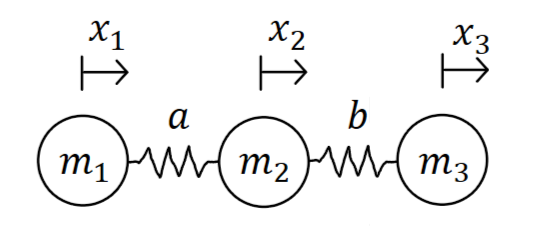
\includegraphics[width=0.7\textwidth, keepaspectratio]{./src/3 Massen System.png}
                        \caption{System mit 3 Massen}
                        \label{fig: 3 Massen System}
                  \end{minipage}
                  \hfill
                  \begin{minipage}[ht]{0.49\linewidth}
                        \centering
                        \includegraphics[width=0.7\textwidth, keepaspectratio]{./src/Kräfte Masse 1D.png}
                        \caption{Kräfte an frei geschnittener Masse}
                        \label{fig: Kräfte Masse 1D}
                  \end{minipage}
            \end{figure}

            Betrachtet man nur die $k$-te Masse, so erhält man die wirkenden Kräfte, wie sie in Abb. \ref{fig: Kräfte Masse 1D} dargestellt wurden.

            Mit dem Prinzip von d'Alembert führt dies auf die Gleichung
            \begin{equation}
                  \label{eqn: Gl für kte Masse}
                  m_k\,\ddot x_k + c_{k-1}\,(x_k-x_{k-1}) - c_k\,(x_{k+1}-x_k) = 0
            \end{equation}

            Man beachte, dass für unbewegliche Masse $m_{k-1}$, also für den Fall, dass
            $$x_{k-1} \equiv 0$$
            (\ref{eqn: Gl für kte Masse}) sich zu
            \begin{equation}
                  \label{eqn: Gl für kte Masse mit Rand links}
                  m_k\,\ddot x_k + c_{k-1}\,x_k - c_k\,(x_{k+1}-x_k) = m_k\,\ddot x_k + (c_{k-1}+c_k)\,x_k -c_k\,x_{k+1} = 0
            \end{equation}
            reduziert.

            In diesem Fall kann die $(k-1)$-te Masse als Rand betrachtet werden, für $k=1$ entspricht (\ref{eqn: Gl für kte Masse mit Rand links}) also genau der Gleichung für die Masse $m_1$ in Abb. \ref{fig: Längsschwinger 1d}.

            Falls man diese Gleichungen für alle n Massen aufstellt, dann können diese zu einer Gleichung der Art

            \begin{equation}
                  \label{eqn: MK Gleichung in 1D}
                  M\,\ddot x + K\,x = 0,\quad M,\ K\in\R^{n\times n}
            \end{equation}
            zusammengefasst werden. Anhand der gewonnenen Gleichung werden die Massen- und Steifigkeitsmatrix abgelesen.

            % Man sieht, dass hier M eine Diagonalmatrix ist, die nur positive Einträge auf der Hauptdiagonalen besitzt.
            % Sie ist somit insbesondere positiv definit, da alle Minoranten positiv sind.

            % Für den zwei-dimensionalen Fall benötigt man $n^2$ Punkt Massen und für jeden Punkt auch 2 Einträge in $x$, da es nun eine Bewegung in x- und in y-Richtung gibt.
            % Somit existieren $2\,n^2$ Einträge in $x$, aber jede Masse besitzt nur 2 Verbindungen mehr, somit wird die Steifigkeitsmatrix \K viel größer, aber auch viel schwächer besetzt.
            
      \section{Ermittlung der Matrizen der Modellprobleme}
            % Nun werden die Massen- und Steifigkeitsmatrix der obigen Systeme berechnet.
            Beginne dazu mit dem System aus Abb. \ref{fig: Längsschwinger 1d}

            Die Gleichung für $m_1$ ist durch (\ref{eqn: Gl für kte Masse mit Rand links}) mit $k=1$ gegeben.
            Für $k=2,\dots, n-1$ gilt (\ref{eqn: Gl für kte Masse}).
            
            Da die Masse $m_n$ durch die rechte Feder mit dem Rand verbunden ist, gilt analog zu oben $x_{n+1} \equiv 0$.
            Man erhält
            $$m_n\,\ddot x_n + c_{n-1}\,(x_n-x_{n-1}) + c_n\,x_n = 0.$$  

            Nach Umstellen folgt:
            \begin{equation}
                  \label{eqn: System GDgl MK 1d}
                  \begin{cases}
                        m_1\ \ddot x_1 + (c_0+c_1)\,x_1 - c_1\,x_2 & = 0   \\
                        m_i\ \ddot x_i - c_{i-1}\,x_{i-1} + (c_{i-1}+c_i)\,x_i -c_i\,x_{i+1} & = 0,\ i=2,...,n-1 \\
                        m_n\ \ddot x_n - c_{n-1}\,x_{n-1} + (c_{n-1}+c_n)\,x_n & = 0
                  \end{cases}
            \end{equation}

            Dieses System kann man zusammenfassen zu:
            $$M\,\ddot x + K\,x = 0,$$
            % damit wird die folgende Matrix quadratischer
            \renewcommand{\arraystretch}{1.5}
            wobei $$M= \text{diag}(m_1,\dots,m_n),\ 
            K = \begin{pmatrix}
                  c_0+c_1 & -c_1 &  &  & 0 \\
                  -c_1 & c_1+c_2 & -c_2 &  &  \\
                   & -c_2 & c_2+c_3 & \ddots &  \\
                    &  & \ddots & \ddots  & -c_{n-1} \\
                   0&  & & -c_{n-1} & c_{n-1}+c_n \\
                  \end{pmatrix}$$

                  
            % wird wieder auf Standard zurückgesetzt
            \renewcommand{\arraystretch}{1}
% Erklärung x? Oder kennt das jeder

% hier muss was über die Eigenschaften gesagt werden
            
            % Für das zwei-dimensionale System kann dieses Verfahren analog angewendet werden. 

      \section{Zusammenhang Eigenwert und Eigenfrequenz}
            Nach der Ermittlung der zugehörigen Matrizen, werden nun die Eigenfrequenzen des Systems bestimmt.
% Eigenkreisfrequenzen?

            Da in diesen Systemen die Massen um ihre Ruhelage schwingen und keine weiteren Kräfte wirken, schwingt jede einzelne Masse harmonisch.
            Nach \cite[S. 380]{maschinendynamikDresig} gilt daher mit $x$ statt $q$:
            $$x(t) = v\,\exp(i\w t),\ \ \ddot x(t) = -\w^2\,v \exp(i\w t)$$
            mit $v=(v_1,...,v_n)$ Vektor der Amplituden und der \zitat{noch unbekannten Eigenkreisfreqenz \w}\cite[S. 380]{maschinendynamikDresig}
            
            Diesen Ansatz kann man in (\ref{eqn: MK Gleichung in 1D}) einsetzen und erhält nach dividieren durch $\exp(i\w t)\footnote{offensichtlich ist die Division wohldefiniert, da $\exp(i\w t)\ne 0\ \forall \w, t\in\R,$}$:
            
            \begin{equation}
                  \label{eqn: verallg EW Problem mit w}
                  (K-\w^2\,M)\,v = 0
            \end{equation}

            Die Gleichung kann ebenfalls in \cite[S. 380]{maschinendynamikDresig} gefunden werden.

            Man will diese Gleichung für $v\ne 0$ lösen, da man sonst eine triviale Lösung erhält, in der keine Masse schwingt.


% braucht man wohl hier noch nicht
            Um (\ref{eqn: verallg EW Problem mit w}) mit $v\ne 0$ zu erfüllen, muss
            $$\det\klammer{K-\w^2\,M} = 0$$
            erfüllt sein.
% nachschlagen, warum das so ist

\chapter{Zählung von Eigenwerten}
\label{sec: EW Zählung}
% vielleicht eher Finden der Zielfunktion nennen
% es fehlt noch: Einführung s und Erklärung, warum nun lambda statt w^2
      
      Nun wende man sich dem Finden einer Zielfunktion zu, die die Anzahl der Eigenwerte auf einem Intervall beschreibt.
      Diese Funktion soll von dem Design-Parameter $s$ (vgl. \cite[S. 2]{hauptteilTkachuk}) abhängen und schlussendlich minimiert werden,
      um ein $s$ aus der zulässigen Menge $\Omega$ zu finden, für welches die Zielfunktion minimal ist, also kein Eigenwert in dem vorgegebenen Intervall liegt.
      \section{mathematische Formulierung}
      Die in diesem Abschnitt erwähnten Schritte stammen aus \cite[S. 2-4]{hauptteilTkachuk}.

      Betrachte das Problem
      $$(K-\w^2 M)x = 0$$
      Falls man das Problem eigenständig betrachtet, so sucht man eine Familie $(\w_j)_j$, die diese Gleichung für ein $x_j \ne 0$ löst.

      Um auf die Form eines Matrix pencils und somit auf die normale Form eines verallgemeinerten Eigenwertproblems zu gelangen, definiere
      $$\lambda_j := \w_j^2$$
% zitat      
      Für das Lösen dieser Gleichung sucht man nun nicht mehr eine Familie $(\w_j)_j$, sondern genau die Eigenwerte des pencils, $\lambda(K,M)$.
      Man beachte aber, dass sich durch die Substitution auch die gegebenen Grenzen verändert haben:
      man will nun, dass keine Eigenwerte des pencils $(\AlamB)$ in dem Intervall $[\lambda_a, \lambda_b]:=[\w_a^2,\w^2_b]$ liegen.

      Eine normale Massematrix, d.h. eine Diagonalmatrix mit ausschließlich positiven Einträgen, ist offenbar regulär.
% warum wichtig
      Definiere nun die Funktion $h$ wie folgt:
      $$h(\lambda):=\1_{[\lambda_a,\lambda_b]}(\lambda)$$

      Da man nur daran interessiert ist, ob ein Eigenwert in dem Intervall liegt oder nicht, definiere

      $$\mu := \sum_{j=1}^{n'} h(\lambda_j)$$

      Obwohl diese Funktion korrekt ist, so gibt es doch einige Schwachstellen, sollte man diese Funktion minimieren wollen:
% wie kann eine Funktion korrekt sein?
      Die Funktion ist nicht stetig differenzierbar und entscheidender: sie ist eine Treppenfunktion, damit sind alle Ableitungen gleich 0, also unbrauchbar für Minimierungsalogrithmen, die mit der Ableitung arbeiten.

      Diese Probleme kann man abfedern, indem man die Funktion auf dem Intervall $[\lambda_a, \lambda_b]$ gewichtet.
% abfedern
      Nutze dazu eine Gewichtungsfunktion, die auf dem ganzen Intervall positiv und konkav ist.
      Diese Funktion sorgt dafür, dass Eigenwerte in der Mitte des Intervalls stärker ins Gewicht fallen
      Nach \cite[S. 3]{hauptteilTkachuk} sei die Funktion
      $$g(z) = -(z-((1+\alpha)\lambda_a -\alpha\lambda_b))(z-((1+\alpha)\lambda_b-\alpha\lambda_a))$$
      sehr geeignet, man könnte aber auch zum Beispiel die Funktion
      $$\Hat g(z) := -(z-(\lambda_a-\alpha))(z-(\lambda_b+\alpha))$$
      nutzen, die die gleichen Eigenschaften besitzt.
      In den Funktionen stellt $\alpha>0$ einen Parameter dar, der dafür sorgt, dass die Funktion auf dem Intervall positiv ist.
      $\alpha$ wird auch \zitat{Inflationsparameter} (vgl. \cite[S. 3]{hauptteilTkachuk}) genannt.
% Inflationsparameter

      Man findet so die erste Funktion, welche man mit Verfahren der Optimierung sinnvoll minimieren könnte:
      $$J(s) = \sum_{j=1}^n g(\lambda_j)h(\lambda_j)$$

      Hier müsste man allerdings jeden Eigenwert zuerst berechnen, um dann diese Formel anzuwenden.
      Auch hängt weder $g$ noch $h$ explizit von $s$ ab, weshalb diese Funktion eher zur Ermittlung der gewichteten Anzahl von Eigenwerten gesehen werden kann, als die tatächliche Zielfunktion, die es zu minimieren gilt.
      Nutze daher die Identität von Futamura, wie sie in Theorem \ref{thrm: IdentitätFutamura} vorgestellt wurde.
      
      Um diese Identität anzuwenden, berachte die Funktion
      $$f(z) = \sum_{j=1}^{n} \frac{1}{z-\lambda_j},$$
      wobei die $\lambda_j$ die Eigenwerte des Matrix pencils $(\AlamB)$ sind.

      Die Funktion besitzt somit eine Polstelle in jedem Eigenwert.

      Nach dem Residuensatz gilt:
      
\chapter{Implementierung}
\label{sec: Programmieren}
      \section{Erklärungen}

      \section{Implementation}

      \section{Grafiken}

\chapter{Verbesserungen}
\label{sec: Verbesserungen}
      \section{Auswertung bisheriger Implementation}

      \section{mögliche Verbesserungen}

      \section{Implementation und Auswertung der verbesserten Programme}

      \section{Approximation der Spur}

\chapter{Auswertung}
\label{sec: Auswertung}

\chapter{Literaturverzeichnis}

      % \begin{figure}[h]
      %       \centering
      %       \begin{minipage}[h]{0.49\linewidth}
      %       \centering
      %       \bilder{"./sources/himmel_und_wolken (www.umweltbundesamt.de)"}
      %       \caption{Betrachter:in auf der Erde}\cite{Himmel}
      %       \label{fig:himmel}
      %       \end{minipage}
      %       \hfill
      %       \begin{minipage}[h]{0.49\linewidth}
      %       \centering           
      %       \bilder{"./sources/erde (www.umweltbundesamt.de)"}
      %       \caption{Betrachter:in im Weltall auf die Erde}\cite{ErdeausWeltall}
      %       \label{fig:ErdeausWeltall}
      %       \end{minipage}
      % \end{figure}

      \printbibliography


%%
%% Erscheint auf letzter Seite
%%
\chapter*{Erkl\"{a}rung}
\thispagestyle{empty}
Hiermit erkl\"{a}re ich, dass ich die am \datum\ eingereichte Bachelorarbeit zum Thema
\emph{\thema} unter Betreuung von \betreuer\ selbstst\"{a}ndig erarbeitet,
verfasst und Zitate kenntlich gemacht habe. Andere als die angegebenen Hilfsmittel
wurden von mir nicht benutzt.

\bigskip \bigskip \bigskip \bigskip \bigskip

Dresden, \datum\ \hfill Unterschrift

\normalsize
\end{document}



